\newpage
\subsubsection{UC3 - Attivazione apprendimento di flusso costante}
\label{sssec:UC3}

\begin{figure}[h!]
  \begin{center}
    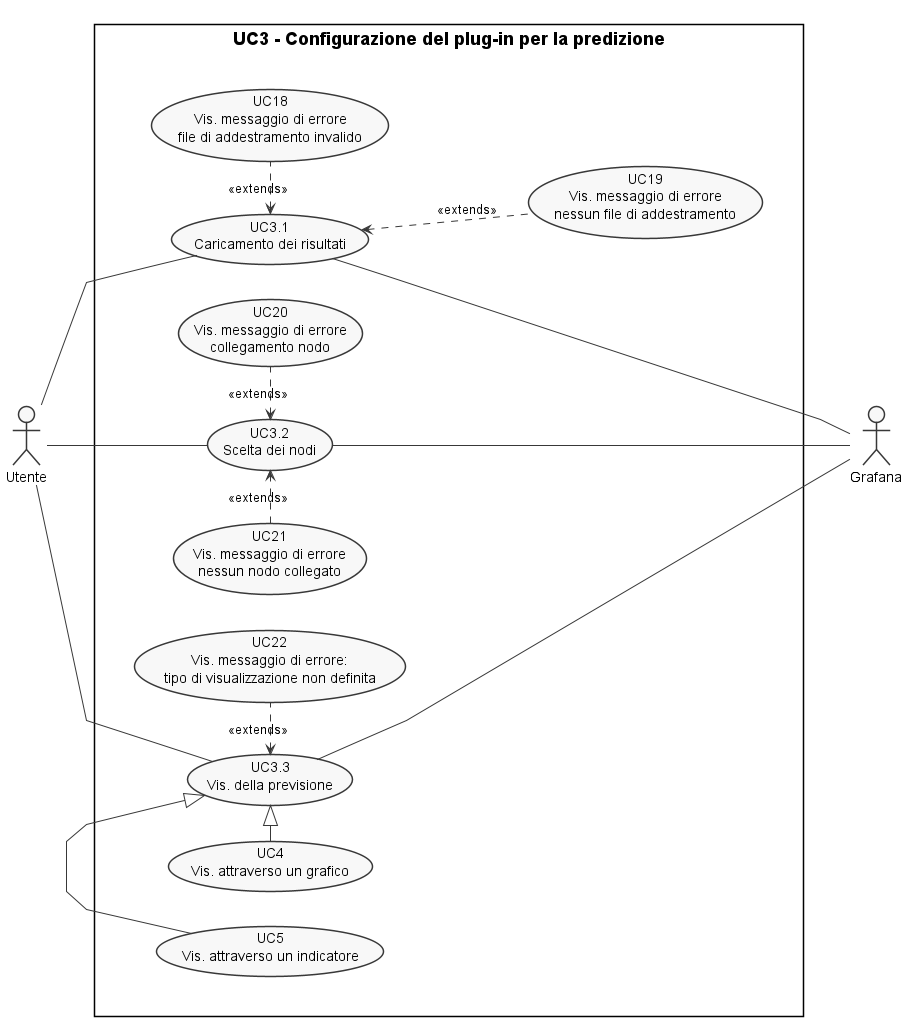
\includegraphics[width=17cm]{uc3.png}\\
    \caption{UC3 - Attivazione apprendimento di flusso costante}%
    \label{fig:uc3}
  \end{center}
  \end{figure}

\begin{itemize}
  \item \textbf{Attore primario}: Utente;
  \item \textbf{Attore secondario}: Grafana;
  \item \textbf{Descrizione}: L'utente decide di attivare l'apprendimento in costante adattamento ai dati rilevati sul campo. Questo porta ad avere un aggiornamento automatico del predittore in base ai nuovi dati ricevuti;
  \item \textbf{Precondizione}:
  \begin{enumerate}
    \item L'utente ha abilitato correttamente il plug-in dalle impostazioni di Grafana;
    \item L'utente ha scelto di attivare l'apprendimento continuo accedendo al pannello dedicato a questo.
  \end{enumerate}
  \item \textbf{Scenario principale}:
  \begin{enumerate}
    \item L'utente seleziona quale algoritmo utilizzare per attivare l'apprendimento costante (UC3.1);
    \item L'utente seleziona su quale sorgente dati effettuare l'apprendimento costante (UC3.2).
  \end{enumerate}
  \item \textbf{Postcondizione}: E' stata attivita la modalità di apprendimento continuo.
\end{itemize}

\paragraph{UC3.1 - Scelta dell'algoritmo da utilizzare}
\label{para:uc3.1}
\begin{itemize}
  \item \textbf{Attore primario}: Utente;
  \item \textbf{Descrizione}: L'utente seleziona l'algoritmo da utilizzare per l'addestramento costante, scegliendo tra RL e SVM;
  \item \textbf{Precondizione}:
  \begin{enumerate}
    \item L'utente ha selezionato il pannello dedicato all'apprendimento di flusso costante;
    \item L'utente ha a disposizione due algoritmi per effettuare l'apprendimento costante.
  \end{enumerate}
  \item \textbf{Scenario principale}: L'utente seleziona l'algoritmo da utilizzare per l'apprendimento costante;
  \item \textbf{Postcondizione}: L'utente ha selezionato l'algoritmo per effettuare l'apprendimento costante, scegliendo tra RL e SVM;
  \item \textbf{Estensione}: UC3.1 viene generalizzato dai casi d'uso UC9 e UC10.
\end{itemize}

\paragraph{UC3.2 - Scelta della sorgente dati da utilizzare}
\label{para:uc3.2}
\begin{itemize}
  \item \textbf{Attore primario}: Utente;
  \item \textbf{Attore secondario}: Grafana;
  \item \textbf{Descrizione}: L'utente seleziona quale sorgente dati utilizzare;
  \item \textbf{Precondizione}: L'utente ha a disposizione un'insieme di dati;
  \item \textbf{Scenario principale}: L'utente sceglie quale sorgente di dati utilizzare per l'apprendimento di flusso costante;
  \item \textbf{Postcondizione}: L'utente ha selezionato quale sorgente di dati utilizzare per l'apprendimento di flusso costante.
\end{itemize}

